%%%%%%%%%%%%%%%%%%%%%%%%%%%%%%%%%%%%%%%%%%%%%%%%%%%%%%%%%%%%%%%%%%%%%%%%%%
% HEADER
%%%%%%%%%%%%%%%%%%%%%%%%%%%%%%%%%%%%%%%%%%%%%%%%%%%%%%%%%%%%%%%%%%%%%%%%%%

\pdfoutput=1

\documentclass[iop, apj, onecolumn]{emulateapj}

\usepackage{xspace}
\usepackage{amsmath}
\usepackage{framed} 
\usepackage{txfonts}
\usepackage{epstopdf}
\usepackage{graphicx}
\usepackage{color}
\usepackage{rotating}
\usepackage{natbib}
\usepackage{ulem}
\usepackage{xspace}
\usepackage[colorlinks=true,urlcolor=blue,linkcolor=blue,citecolor=blue]{hyperref}

\special{papersize=8.5in,11in}
\setlength{\pdfpageheight}{\paperheight}
\setlength{\pdfpagewidth}{\paperwidth}

%\input{commands}
%\input{macros}
%\input{citation_fix}

\shorttitle{Smoothing filter}
\shortauthors{More, S. \& others}

%\journalinfo{The Astrophysical Journal, {\rm 789:1 (18pp), 2014 July 1}}
%\submitted{Received 2014 January 6; accepted 2014 April 14; published 2014 June 9}
\slugcomment{Only submitted to the arXiv}

\begin{document}

%%%%%%%%%%%%%%%%%%%%%%%%%%%%%%%%%%%%%%%%%%%%%%%%%%%%%%%%%%%%%%%%%%%%%%%%%%
% EPS OR PDF FIGURES
%%%%%%%%%%%%%%%%%%%%%%%%%%%%%%%%%%%%%%%%%%%%%%%%%%%%%%%%%%%%%%%%%%%%%%%%%%

%%%%%%%%%%%%%%%%%%%%%%%%%%%%%%%%%%%%%%%%%%%%%%%%%%%%%%%%%%%%%%%%%%%%%%%%%%
% TITLE ETC
%%%%%%%%%%%%%%%%%%%%%%%%%%%%%%%%%%%%%%%%%%%%%%%%%%%%%%%%%%%%%%%%%%%%%%%%%%

\title{Extending the Savitzky Golay smoothing filter to data with covariant
errors}
\author{
Surhud More \altaffilmark{1}
}

\affil{
$^1$ Kavli Institute for the Physics and Mathematics of the Universe (WPI),
Tokyo Institutes for Advanced Study, The University of Tokyo,\\ 5-1-5 Kashiwanoha, Kashiwa-shi, Chiba, 277-8583, Japan;{\tt surhud.more@ipmu.jp}\\
}

%%%%%%%%%%%%%%%%%%%%%%%%%%%%%%%%%%%%%%%%%%%%%%%%%%%%%%%%%%%%%%%%%%%%%%%%%%
% ABSTRACT
%%%%%%%%%%%%%%%%%%%%%%%%%%%%%%%%%%%%%%%%%%%%%%%%%%%%%%%%%%%%%%%%%%%%%%%%%%

\begin{abstract}
Digital filters need to be commonly applied to noisy data for the purpose of
smoothing it and allowing a less noisy computation of the derivative. The
commonly used filter developed by Savitzky \& Golay based on a simplified least
squares procedure assumes no or equivalently equal errorbars on all data points.
I present a simple extension of this filter to unequal errors with covariance, a
typical case for many scientific datasets. A python implementation has been made
available at http://github.com/surhudm/savitzky\_golay\_with\_errors for ease of
use.
\end{abstract}

\keywords{}

%%%%%%%%%%%%%%%%%%%%%%%%%%%%%%%%%%%%%%%%%%%%%%%%%%%%%%%%%%%%%%%%%%%%%%%%%%
% INTRODUCTION
%%%%%%%%%%%%%%%%%%%%%%%%%%%%%%%%%%%%%%%%%%%%%%%%%%%%%%%%%%%%%%%%%%%%%%%%%%

\section{Introduction}
\label{sec:intro}

The presence of noise in scientific data is unavoidable. The removal of noise
from data without degrading the underlying information is fundamental to
obtaining physical insights from the data. In particular smoothing is crucial in
the absence of detailed physical models, in order to gain some phenomenological
understanding of the observed phenomenon. 

\citet{SG1964} presented a simple numerical procedure for this purpose. Consider
data drawn from $y_i=f(x_i)+\epsilon$, where $\epsilon$ represents the noise,
and the index $i$ runs over the $N$ data points. The algorithm presented by
\citet{SG1964} considers a moving window (an odd integer, $2m+1$) centered
around the data point to be smoothed. The data is approximated as a polynomial
of degree $n$ around this point, whose parameters are determined using a least
squares procedure. The polynomial is then used to estimate the smoothed version
of the data. 
\begin{equation}
        y_{\rm SG}(x_i) = f^{\rm poly}_{n}(x_i|{y_i', i'\in[i-m,i+m]})
\end{equation}
The solution obtained by the minimization of least squares presented in
\citet{SG1964} does not use the estimates of the errors on the data (or
equivalently assumes equal errors on all data points without any covariance).
This results in a simple solution for the problem where the data has to be
convolved with a set of predetermined integers. This simple solution has been
implemented in many numerical libraries including python's numpy
(savgol\_filter) and has been used in the literature quite often (ADS suggests
1470 citations to the paper, Google scholar which perhaps tracks citations in
all the scientific fields suggests over 9000).

Although touted to be an optimal smoothing solution, the assumption of equal and
independent errors is quite rarely satisfied in real data. Therefore, I simply
recommend and extend this filter to use the errors whenever they are available.
I will show that in the case of data with heteroscedastic (unequal) errors,
using these errors provides a much better description of the underlying signal
than the traditional Savitzky-Golay filter.

\section{Mathematical background behind the implementation}

The mathematical machinery behind the Savitzky Golay smoothing filter reduces to
the problem of fitting a $n^{\rm th}$ degree polynomial to a set of $(2m+1)$
data points with errors. This is a well known problem in linear algebra, and we
present the simple solution for pedagogical purposes. The $\chi^2$ metric for
the polynomial fitting problem with covariant errors is given by
\begin{equation}
        \chi^2 = ({\bf y}-{\bf y}_{\rm model}[{\bf x}])^T {\bf C}^{-1}
                ({\bf y}-{\bf y}_{\rm model}[{\bf x}])\,,
\end{equation}
where
\begin{equation} 
        {\bf y}_{\rm model}({\bf x}) = {\bf V}({\bf x}){\bf a}\,.
\end{equation}
Here, ${\bf V}$ denotes the Vandermonde matrix, ${\bf a}$ denotes the $(n+1)$
coefficients of the $n^{\rm th}$ degree polynomial, and we seek those
coefficients which minimize the $\chi^2$. Differentiating with respect to ${\bf
a}$ gives
\begin{eqnarray}
        \frac{\partial \chi^2}{\partial {\bf a}} &=& -{\bf y}^T {\bf C}^{-1} {\bf
        V} - {\bf V}^T {\bf C}^{-1} {\bf y} + {\bf a}^T {\bf
        V}^T {\bf C}^{-1} {\bf V} + {\bf V}^T {\bf C}^{-1} {\bf V} {\bf a} \\
        &=& - {\bf V}^T {\bf C}^{-1} {\bf y} + {\bf V}^T {\bf C}^{-1} {\bf V}
        {\bf a}\,,
\end{eqnarray}
where the second equality relies on the symmetry of the inverse covariance
matrix which results in the first and the last two terms being equal. Equating
the derivative to zero yields
\begin{equation}
        {\bf a} = \left[ {\bf V}^T {\bf C}^{-1} {\bf V}\right]^{-1} {\bf
        V}^T{\bf C}^{-1} {\bf y}
\end{equation}

We provide a convenient python routine which implements the above equations in
case a covariance matrix is passed and returns the optimally filtered data.  For
the special case of independent errors, the routine utilizes the standard
polynomial fitting algorithm in the numpy library. This routine has been made available online.
\footnote{http://github.com/surhudm/savitzky\_golay\_with\_errors}

As a simple example let us consider data drawn from a sinusoid with
heteroscedastic errors. The traditional Savitzky Golay fit is compared to the
improved version in the left panel of Figure~\ref{fig:improve}. The left hand
panel shows a similar case, but where the errors on the data further include
covariance. The covariance is chosen such that the strength of the
cross-correlation between two points is inversely proportional to the square of
the difference in their abscissa. The $\chi^2$ reported in the lower row of
each of the panels are computed with respect to the noiseless values at each
point but using the covariance of the noisy data, i.e., $\chi^2=({\bf y}_{\rm
smooth}-\sin[{\bf x}])^T {\bf C}^{-1} ({\bf y}_{\rm
smooth}-\sin[{\bf x}])$. It is clear that the traditional smoothing
filter is pulled away from the real solution by outliers which also have larger
errors associated with them. By accounting for these errors and their
covariance, the improved filter presented in this work, provides a better
alternative.

\begin{figure} 
        \centering{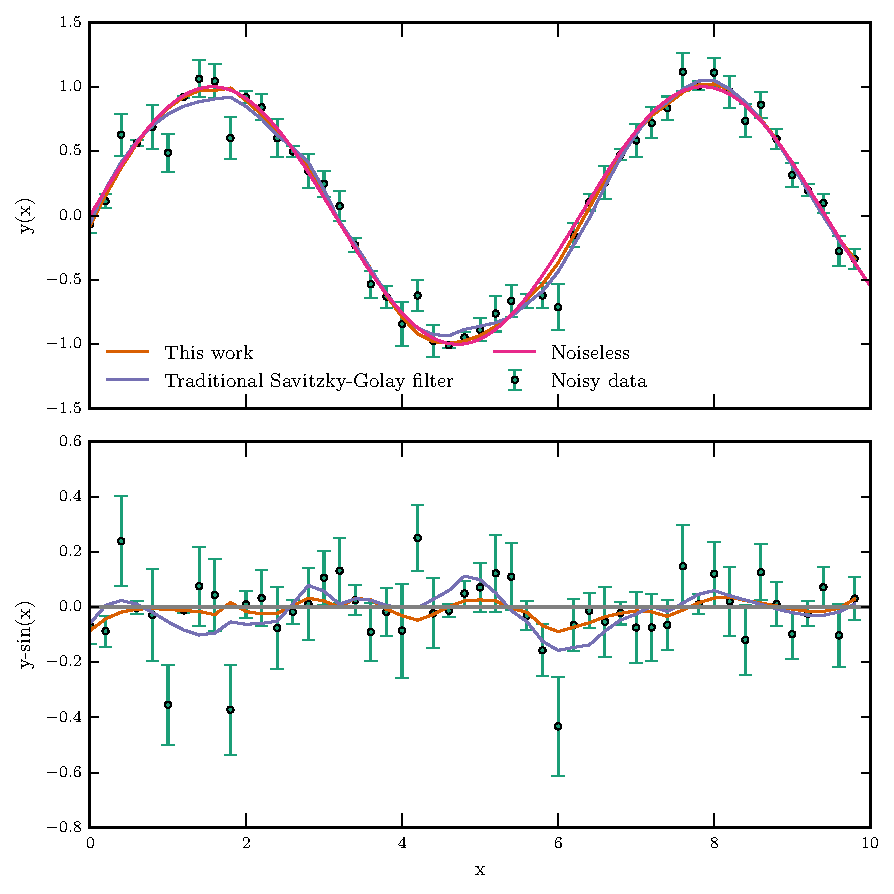
\includegraphics[scale=0.5]{Test_Sine.pdf}}
        \centering{\includegraphics[scale=0.5]{Test_Sine_wcov.pdf}}
\caption{
        Data from a noisy $sin(x)$ curve filtered using the traditional
        Savitzky-Golay filter which assumes equal errors compared to the
        improved filter presented in this work which uses the actual errors on
        the data. Both the filters assume a window of 15 points and a fourth
        degree polynomial to fit the data. The improved filter performs
        significantly better and gives a much better representation of the data.
}
\label{fig:improve}
\end{figure}


%%%%%%%%%%%%%%%%%%%%%%%%%%%%%%%%%%%%%%%%%%%%%%%%%%%%%%%%%%%%%%%%%%%%%%%%%%
% BIBLIOGRAPHY
%%%%%%%%%%%%%%%%%%%%%%%%%%%%%%%%%%%%%%%%%%%%%%%%%%%%%%%%%%%%%%%%%%%%%%%%%%

\bibliographystyle{apj}
\bibliography{sf}
\end{document}
